\section{Einordnung}
\begin{itemize}
	\item Wie sieht das Schichtenmodell vom Beginn der Vorlesung inzwischen aus?
	\item Welche Strukturen werden in den jeweiligen Schichten verwendet?
	\item Wie wird jede Schicht von der darüber liegenden adressiert? Wie adressiert sie selbst?
\end{itemize}

\begin{solution}
Ein paar Stichworte zur Diskussion (am Ende sollte eine Grafik ähnlich der auf Folie~\SchichtVLFuenf~oder~\SchichtVLSechs~entstanden sein):
\begin{itemize}
	\item interne Satzschnittstelle
	\item blockorientierte Schnittstelle
	\item Satzverwaltung
	\item Externspeicherverwaltung
	\item Kanalkommandos
\end{itemize}

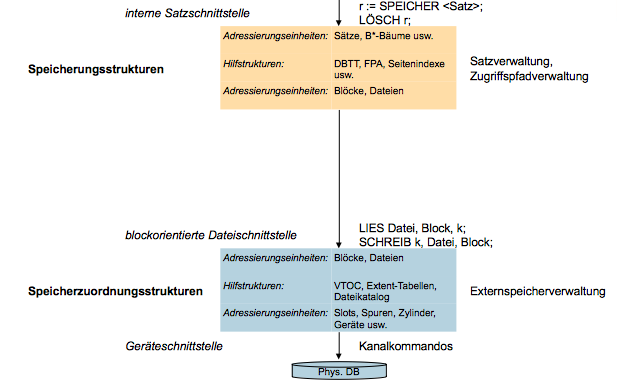
\includegraphics[width=14cm]{Pictures/Ue06_Aufgabe3_1.png}

Einfügen einer seitenorientierten Pufferschnittstelle, Details im nächsten Übungsblatt:

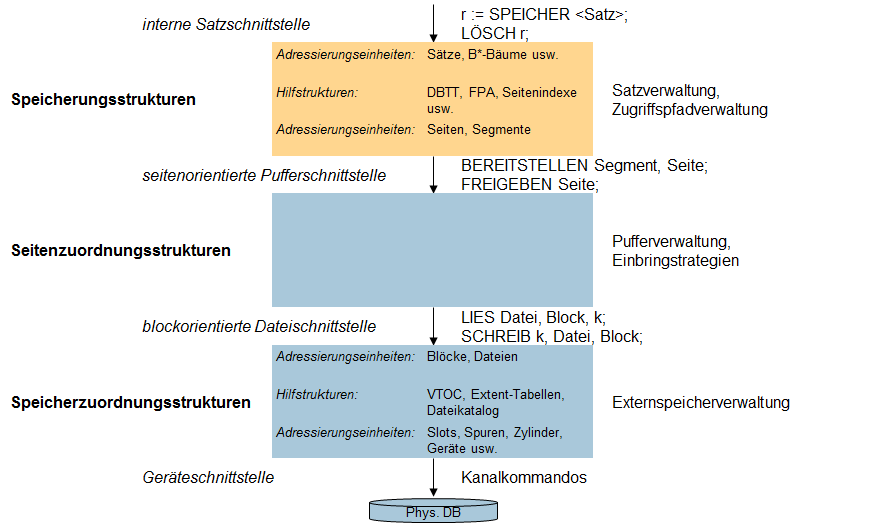
\includegraphics[width=14cm]{Pictures/Ue06_Aufgabe3_2.png}

\end{solution}
